\section{Part 1}

Part one of step four required students to perform a rudimentary read-write
exercise using PSpice.  Using a~``RAM8kX8break'' RAM element paired with
several digital value generators, values were written to each of two different
memory addresses.

\subsection{Schematic}
As the lab instructions provided a functioning schematic for this system, it
has been reproduced here in Figure~\ref{f:schem1}.
%
\begin{figure}[H]
\centering
	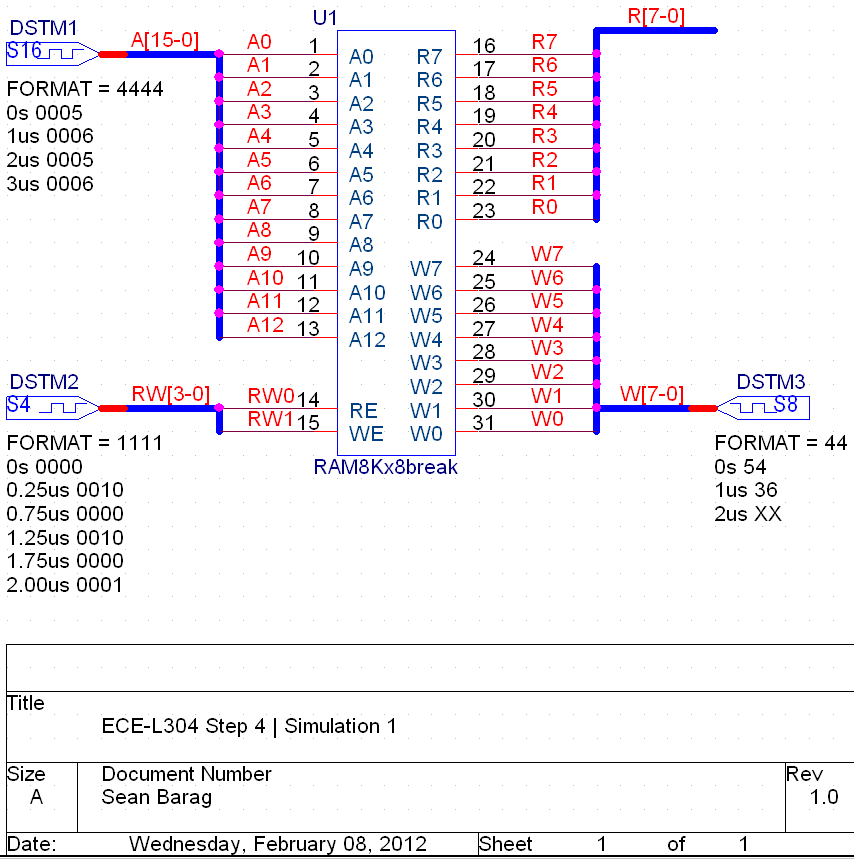
\includegraphics[width=.8\textwidth]{img/shot/schem1.png}
	\parbox{.8\textwidth}{
	\caption[Part 1 Schematic]{PSpice schematic for the circuit simulated in
	part one of step four.}
	\label{f:schem1}}
\end{figure}
%
The system writes the hex values \ttt{0x54} and \ttt{0x36} to the registers
located at \ttt{0x05} and \ttt{0x06}, respectively.  The values at these
locations are then read back to the \ttt{R} bus in the same sequence in which
they were written.

\subsection{Simulation}
For the sake of such a simple example, each read and write operation takes
just~\SI{1}{\micro\second}.  This allowed the student to simulate the circuit
over a convenient~\SI{4}{\micro\second} period while monitoring the values at
each data bus.  The plot produced by PSpice for this simulation is shown in
Figure~\ref{f:schem1plot}.
%
\begin{figure}[H]
\centering
	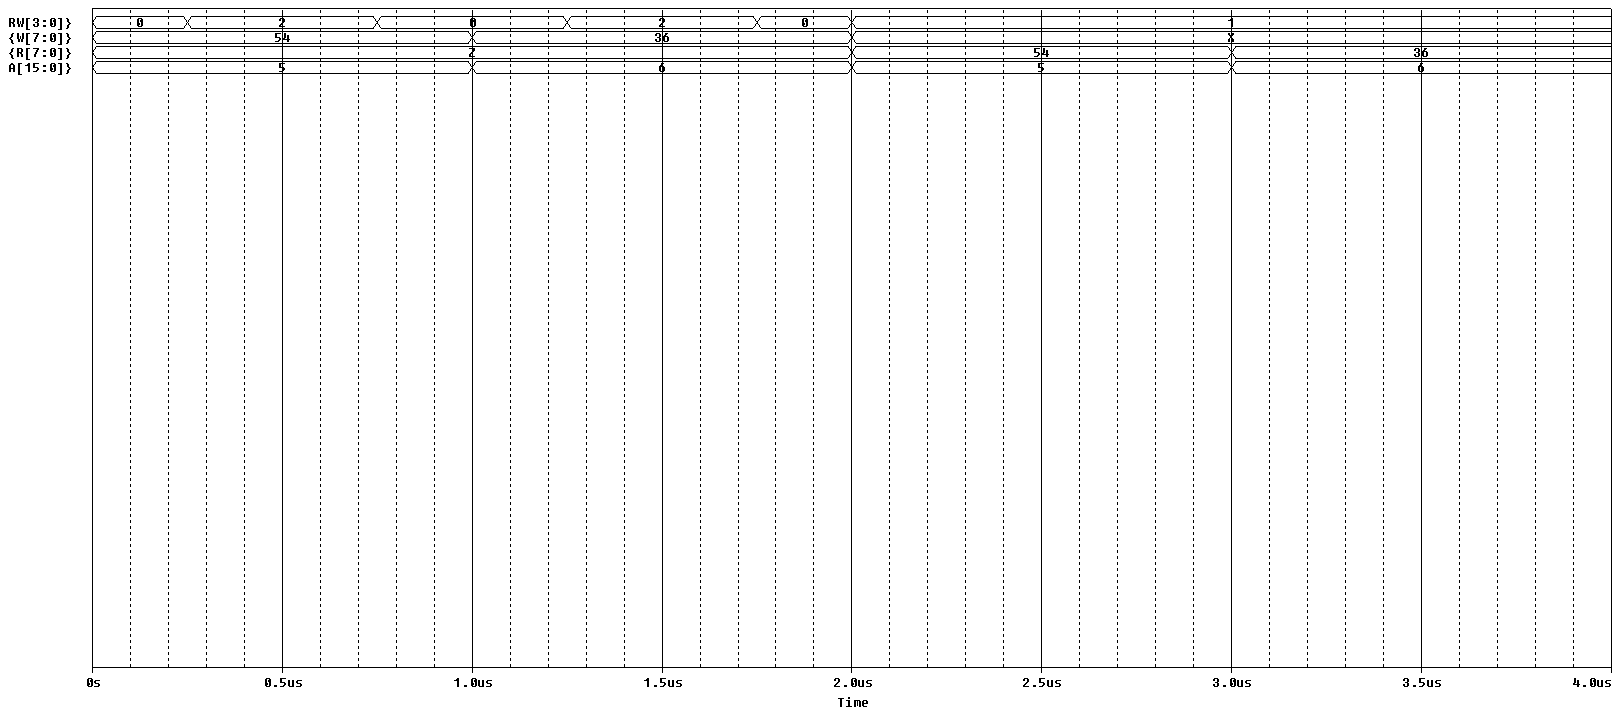
\includegraphics[width=.8\textwidth]{img/shot/sim1_plot.png}
	\parbox{.8\textwidth}{
	\caption[Part 1 Simulation Results]{Results of simulating the schematic
	shown in Figure~\ref{f:schem1} for~\SI{4}{\micro\second}.  A larger version
	of this figure is available in appendix Figure~\ref{f:schem1plot_big}.}
	\label{f:schem1plot}}
\end{figure}
%
The output of a hypothetical address generator is connected to the \ttt{A}
register, which changes value once per millisecond.  Note that the duplicate
addresses are present so that the system can read values from said addresses
after storing the value of \ttt{W} during the first occurrence of each address.
Reading and writing are enabled by the  \ttt{RW} register.  As the timing in
Figure~\ref{f:schem1} implies, writing is enabled for~\SI{0.5}{\micro\second}
across the center of each value from the \ttt{A} bus (i.e. from~$i +
\SI{0.25}{\micro\second}$ to~$i + \SI{0.75}{\micro\second}$.
After~\SI{2}{\milli\second}, \ttt{RW} enables reading for an infinite amount of
time.  As a result of these characteristics, it is safe to conclude that the
system follows all applicable read/write rules.

Figures~\ref{f:schem1plot} and~\ref{f:schem1plot_big} show that the system
correctly reads back the data it writes.  As such, the schematic can be
considered fully functional.
